\subsection{Round 1 Problems}

Solutions can be found in Section~\ref{S::2021-O-1}.

\begin{enumerate}
    \hyperrefitem[A::2021-O-1-1] It is given that $\dfrac\pi2 < \b < \a < \dfrac{3\pi}{4}$, $\cos{\a - \b} = \dfrac{12}{13}$ and $\sin{\a + \b} = -\dfrac35$. Find $\floor{\abs{2021\sin{2\a}}}$.
    \hyperrefitem[A::2021-O-1-2] Find the number of solutions of the equation $\abs{x - 3} + \abs{x - 5} = 2$.

    \textit{(Note: If you think that there are infinitely many solutions, enter your answer as ``99999''.)}
    \hyperrefitem[A::2021-O-1-3] Evaluate $1 \times 2 \times 3 + 2 \times 3 \times 4 + 3 \times 4 \times 5 + \cdots + 10 \times 11 \times 12$.
    \hyperrefitem[A::2021-O-1-4] It is given that the solution of the inequality $\sqrt{81 - x^4} \leq kx + 1$ is $a \leq x \leq b$ with $b - a = 2$, where $k > 0$. Determine $\floor k$.
    \hyperrefitem[A::2021-O-1-5] The figure below shows a cross that is cut out from a $10 \times 9$ rectangular board.

    \begin{center}
        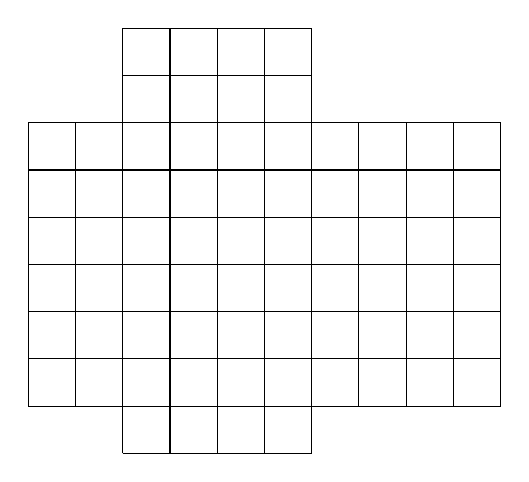
\begin{tikzpicture}[scale=0.6]
            \foreach \y in {1, 2, ..., 7}{
                \draw (0, \y) -- (10, \y);
            }

            \foreach \y in {0, 8, 9}{
                \draw (2, \y) -- (6, \y);
            }

            \foreach \x in {0, 1, 7, 8, 9, 10}{
                \draw (\x, 1) -- (\x, 7);
            }

            \foreach \x in {2, 3, ..., 6}{
                \draw (\x, 0) -- (\x, 9);
            }

        \end{tikzpicture}
    \end{center}
    
    Find the total number of rectangles in the above figure.

    \textit{(Note: A square is a rectangle.)}
    \hyperrefitem[A::2021-O-1-6] Consider all polynomials $P(x, y)$ in two variables such that $P(0, 0) = 2020$ and for all $x$ and $y$, $P(x, y) = P(x + y, y - x)$. Find the largest possible value of $P(1, 1)$.
    \hyperrefitem[A::2021-O-1-7] In the three-dimensional Cartesian space with $\vec i$, $\vec j$ and $\vec k$ denoting the unit vectors along three perpendicular directions in a clockwise manner, the line $l$ with equation given by $\vec r \crossp (\vec i + 2 \vec j + 3 \vec k) = 5\vec i - 13\vec j + 7\vec k$ intersects the plane $\Pi$ with equation $x + y + z = 16$ at the point $(a, b, c)$. Find the value of $a + b + c$.
    \hyperrefitem[A::2021-O-1-8] Find the minimum value of $(x + 7)^2 + (y + 2)^2$ subject to the constraint $(x-5)^2 + (y-7)^2 = 4$.
    \hyperrefitem[A::2021-O-1-9] Find the largest possible value $\a^4 + \b^4 + \g^4$ among all possible sets of numbers $(\a, \b, \g)$ that satisfy the equations
    \[\begin{aligned}
        \a + \b + \g &= 2\\
        \a^2 + \b^2 + \g^2 &= 14\\
        \a^3 + \b^3 + \g^3 &= 20.
    \end{aligned}\]
    \hyperrefitem[A::2021-O-1-10] If $p$ is the product of all the non-zero real roots of the equation \[\sqrt[9]{x^7 + 30x^5} = \sqrt[7]{x^9 - 30x^5},\] find $\floor{\abs{p}}$.
    \hyperrefitem[A::2021-O-1-11] Let $S$ be the sum of a convergent geometric series with first term 1. If the third term of the series is the arithmetic mean of the first two terms, find $\floor{3S + 4}$.
    \hyperrefitem[A::2021-O-1-12] Given that $\sin \a + \sin \b = \dfrac1{10}$, and $\cos \a + cos \b = \dfrac19$, find $\floor{\tan^2{\a + \b}}$.
    \hyperrefitem[A::2021-O-1-13] Determine the number of positive integers that are divisible by 2021 and has exactly 2021 divisors (including 1 and itself).
    \hyperrefitem[A::2021-O-1-14] Let $S = \displaystyle\sum_{k=0}^{25} \binom{100}{4k} - 2^{98}$. Find $\floor{\abs{\dfrac{S}{2^{48}}}}$.
    \hyperrefitem[A::2021-O-1-15] Assume that $ABC$ is an acute triangle with $\sin{A + B} = \dfrac35$ and $\sin{A-B} = \dfrac15$. If $AB = 2022(\sqrt6 - 2)$, determine $\floor h$, where $h$ is the height of the triangle from $C$ on $AB$.
    \hyperrefitem[A::2021-O-1-16] Let $a_1, a_2, \cdots$ be a sequence with $a_1 = 1$ and $a_{n+1} = \dfrac{n+2}{n} S_n$ for all $n = 1, 2, \cdots$, where $S_n = a_1 + a_2 + \cdots + a_n$. Determine the minimum integer $n$ such that $a_n \geq 2021$.
    \hyperrefitem[A::2021-O-1-17] Each card of a stack of 101 cards has one side coloured red and the other coloured blue. Initially all cards have the red side facing up and stacked together in a deck. On each turn, Ah Meng takes 8 cards on the top, flip them over, and place them to the bottom deck. Determine the minimum number of turns required so that all the cards have the red sides facing up again.
    \hyperrefitem[A::2021-O-1-18] Let $ABC$ be a triangle with $AB = 10$ and $\dfrac{\cos A}{\cos B} = \dfrac{AC}{BC} = \dfrac43$. Let $P$ be a point on the inscribed circle of triangle $ABC$. Find the largest possible value of $PA^2 + PB^2 + PC^2$.
    \hyperrefitem[A::2021-O-1-19] A basket contains 19 apples labelled by the numbers $2, 3, \ldots, 20$, and 19 bananas labelled by the numbers $2, 3, \ldots, 20$. Ah Beng picks $m$ apples and $n$ bananas from the basket. However, he needs to ensure that for any apple labelled $a$ and any banana labelled $b$ that he picks, $a$ and $b$ are relatively prime. Determine the largest possible value of $mn$.
    \hyperrefitem[A::2021-O-1-20] Let $p(x) = ax^2 - bx + c$ be a polynomial where $a$, $b$, $c$ are positive integers and $p(x)$ has two distinct roots in $(0, 1)$. Determine the least possible value of $abc$.
    \hyperrefitem[A::2021-O-1-21] In the triangle $ABC$, $\angle A > 90\deg$, the incircle touches the side $BC$ and $AC$ at $A_1$ and $B_1$ respectively. The line $A_1 B_1$ meets the extension of $BA$ at $X$ such that $CXB = 90\deg$. Suppose $BC^2 = AB^2 + BC \cdot AC$. Find the size of $\angle A$ in degrees.
    \hyperrefitem[A::2021-O-1-22] Find the number of positive integers $n$ such that $7n-16$ divides $n \cdot 13^{2019}$.
    \hyperrefitem[A::2021-O-1-23] In the acute triangle $ABC$, $P$ is a point on $AB$, $Q$ is a point on $AC$ such that $BP + CQ = PQ$. The bisector of $\angle A$ meets the circumcircle of the triangle $ABC$ at the point $R$ distinct from $A$. Suppose $\angle PRQ = 52.5\deg$. Find the size of $\angle BAC$ in degrees.
    \hyperrefitem[A::2021-O-1-24] Let $S = \displaystyle\int_{-\infty}^\infty e^{-\frac12 x^2} \d x$. Determine the value of $\floor{S^2}$.
    \hyperrefitem[A::2021-O-1-25] Let $p$, $q$, $r$ be positive numbers with $p-r= 4q$ and $a_1, a_2, \cdots$ and $b_1, b_2, \cdots$ be two sequences defined by $a_1 = p$, $b_1 = q$ and for $n \geq 2$, \[a_n = pa_{n-1}, \quad b_n = qa_{n-1} + rb_{n-1}.\] Find the value of $\displaystyle\lim_{n \to \infty} \dfrac{\sqrt{a_n^2 + (3b_n)^2}}{b_n}$.
\end{enumerate}
